\chapter[Experimental]{Experimental}



{
% Los objetivos no estan diferenciados entre generales y especıficos.
% Se presentan procesos que validan el trabajo comparando con otros metodos del estado del arte. 
% Se presenta una validacion deparametros,y todas las dimensiones que fueron planteadas son exploradas en profundidad.
% Se detalla y explica la recoleccion (de aplicar) y analisis de da- tos y resultados.
% Se distinguen los resultados segun las variables investigadas, y se examinan en virtud de lo explicado en el marco teorico.
%Se interpretan con claridad (es decir, se consideran distintos factores y anteceden- tes descritos hasta el momento) los resultados obtenidos.
}

Lo que se busca es usar como un modelo de navegación creado con algoritmo de compresión basado en Lempel Ziv  y usarlo como un modelo  predicción. Se usará para predecir secuencias finitas discretas de accesos web. Al momento de generar el árbol este creará una representación Trie de un diccionario de símbolos, el cual utilizaremos para poder hacer predicciones.

En base a lo anterior y teniendo funcionando el algoritmo para crear un modelo de predicción, se integrará con el servidor de Machine Learning Prediction.IO que ya se ha explicado anteriormente.



Usaremos la misma API que ofrece Prediction.IO para poder realizar las evaluaciones de nuestras métricas propuestas, dado el dominio de nuestro problema la métrica a usar será Accurracy (Exactitud) frente a distintas porciones de datos.

	%- Cross validation: This method is generally applied in machine-learning evaluation [14]. In our experiments, we performed a K-fold cross validation with k = 10. In this way, our dataset is 10 times split into 10 different sets of learning (90 
	% of the total dataset) and testing (10 % of the total data).
	%-Learning the model: We accomplished the learning step using different learning algorithms depending on


Con el dataset que tenemos haremos variadas pruebas para ver métricas como Accurracy, usaremos Cross Validation en distintos escenarios.





\subsection{Ambientes Experimental}

Para los ambientes experimentales se han dispuestos dos máquinas para realizar las pruebas. 

\subsubsection{Máquinas}
	\begin{itemize}
		\item Procesador 2,8 GHz Intel Core i7, 16 GB de Memoria RAM y Sistema Operativo OSX
		\item Procesadores Intel Xeon E5-2670 v2 (Ivy Bridge) de alta frecuencia 32 vCPU, 244 GB de Memoria RAM y Sistema Operativo Ubuntu 14.14 
	\end{itemize}

\subsubsection{Software}

	\begin{itemize}
		\item C++11
		\item Java  1.8
		\item Java(TM) SE Runtime Environment (build 1.8)
		\item Java HotSpot(TM) 64-Bit Server VM (build $25.51-b03$, mixed mode)
		\item Scala code runner version 2.11.7 -- Copyright 2002-2013, LAMP/EPFL
		\item SBT 0.13.9 
		\item Python 2.7.10
		\item GNU bash 3.2.57 $(x86_64-apple-darwin15)$
		\item Prediction.IO 0.9.4
		\item Elasticsearch 1.4.4	
		\item Apache Spark-1.4.1
		\item Hbase 1.0.0
		\item Zookeeper 
	\end{itemize}









El motor de predicción es Prediction.IO, como se ha señalado anteriormente  es un framework para deployar servidor con algoritmos de Maquians de Aprendizaje, Decission Tree, K-Means, RNN y todos los algortimos ofrecidos por la suite de Apache Spark y MLib. % Colocar unos lindos links para hacer publicidad a esto

Para desarrollar un motor que se intrege con \emph{PIO} se deberá seguir el patrón \emph{DASE} y crear un modelo con persistencia en memoria que nos permita un acceso rápido a las consultas a las predicciones.


Usaremos \emph{SBT} para orequestar todas las liberias que se requieran como dependencia. Inherentemente usaremos Java, ya que el lenguaje Scala corre sobre la Java Virtual Machine. Prediction.IO no solo ocupa Scala, adicionalmente provee el uso de Apache Spark con sus librerías de MLIB (Machine Learning Library), Zookeeper, Hbase (Hadoop) y Elasticsearch. Hemos utilizado Python para realizar un cliente por linea de comando en el cual poder hacer pruebas y adicionalmente hacer un cliente que realice la carga de eventos desde nuestro set de datos experimental. Para mayor referencia de los clientes python ver los fuentes en los anexos.





\subsection{Datos Experimentales}
% Cita a Rkonow Claude & Navarro

Se usará las secuencias disponibles de acceso web pública de los sitios MSNBC. El set de datos provienen de los registros de un servidor IIS (Internet Information Services) msnbc.com de un día completo de la fecha  28 de Septiembre de 1999. 
Contiene secuencias de acceso web de 989,818 usuarios con un promedio de 5,7  categorías Página web visitas por secuencia, el tamaño de letras de este conjunto de datos es $\sigma \ = 17$.


Ejemplo de estructura de Dataset MSNBC :
\vspace{1cm}

\begin{lstlisting}[frame=single,basicstyle=\ttfamily\tiny,]
% Different categories found in input file:

frontpage news tech local opinion on-air misc weather msn-news health living business msn-sports sports summary bbs travel


% Sequences:

A A 
B 
C B B D B B B C C 
E 
A 
F 
A A 
F 
F G G G F F H H H H 
F I D D D J C J E J D D D 
A A A K A A A 
L L 
A A 
H H H H H H 
\end{lstlisting}





Utilizaremos un simple programa en C++ para filtrar y listar los dataset y transformarlos a símbolos, caracteres en mayúscula, por ejemplo:

	
	\begin{lstlisting}[frame=single,basicstyle=\ttfamily\tiny,]
	1 1 
	2 
	3 2 2 4 2 2 2 3 3 
	5 
	1 
	6 
	1 1 
	6 
	6 7 7 7 6 6 8 8 8 8 
	6 9 4 4 4 10 3 10 5 10 4 4 4 
	\end{lstlisting}


 Ejemplo de sub-dataset creados:

%@TODO: Ver como hacer mas pequeño el dataset.
\begin{itemize}
	\item Secuencias de webaccess con sesiones de más de 5 secciones web visitadas
	\item Secuencias de webaccess con sesiones de más de 10 secciones web visitadas
	\item Secuencias de webaccess con sesiones de más de 100 secciones web visitadas
	\item Secuencias de webaccess con sesiones equivalentes a 10 secciones web visitadas
	\item Secuencias de webaccess con sesiones menores a 5 secciones web visitadas
\end{itemize}


Trabajaremos con 1.000.000 de registros de los cuales hemos realizados distintas subconjuntos para hacer una validación cruzada:

\begin{itemize}
	\item 10 Sesiones de usuarios
	\item 100 Sesiones de usuarios
	\item 500 Sesiones de usuarios
	\item 1.000 Sesiones de usuarios
	\item 5.000 Sesiones de usuarios
	\item 10.000 Sesiones de usuarios
	\item 50.000 Sesiones de usuarios
	\item 100.000 Sesiones de usuarios
	\item 500.000 Sesiones de usuarios
	\item 750.000 Sesiones de usuarios
	\item 1.000.000 Sesiones de usuarios
\end{itemize}


Es importante señalar que la división de nuestro set de datos es debido a que no conocemos la naturaleza de los mismo, pero con nuestro modelo podemos hacer un estudio para ir detectando patrones que puedan ser claves para medir el rendimiento en función a los criterios de volumen de datos versus el Accurracy(Exactitud).






\begin{table}[]
	\centering

	\label{table-list-symbol}
	\begin{tabular}{cl}
		Page       & Symbol \\ \cline{1-2}
		frontpage  & A      \\
		news       & B      \\
		tech       & C      \\
		local      & D      \\
		opinion    & E      \\
		on-air     & F      \\
		misc       & G      \\
		weather    & H      \\
		msn-news   & I      \\
		health     & J      \\
		living     & K      \\
		business   & L      \\
		msn-sports & M      \\
		sports     & N      \\
		summary    & O      \\
		bbs        & P      \\
		travel     & Q      \\ 
	\end{tabular}
	\caption{Para poder interpretar la entrada anterior se debe tener esta relación de símbolos con respecto a las páginas}
\end{table}





\subsection{Experimentos con Nuestro Modelo}


\subsubsection{Sesiones con un valor mínimo de visitas a secciones}

Dentro de nuestro experimentos para probar la exactitud de nuestro modelo podemos demostrar que al tener una menor cantidad de secciones visitadas, la probabilidad de no acertar crece considerablemente.


Sea la siguiente sesión de un usuario 
$\{A , B , A  \}  $ para un alfabeto $\Sigma=\{A,B,C,D,E,F,G,H,I,J,K,L,M,N,O,P,Q \} $


	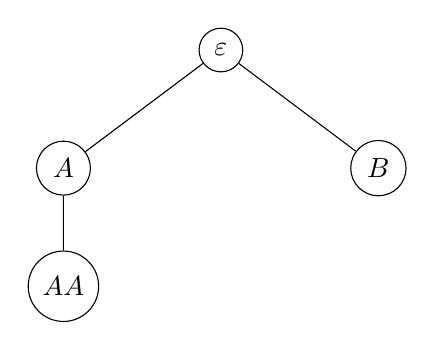
\begin{tikzpicture}[level/.style={sibling distance=40mm/#1}]
	\node [circle,draw] (epsilon){$\varepsilon$}
		child { node [circle,draw] (A) {$A$} 
				child { node[circle,draw](AA){$AA$}  }
			}
		child {node [circle,draw] (B) {$B$} }
	;
	
	\end{tikzpicture}


Como usted puede ver a menor cantidad de símbolos en la sesión estos generan un árbol de menor altura y menos nodos, cada nodo como se ha señalado en el capitulo 4 representa un visita a una sección en particular de la web de MSNBC, pero al ser un sesión tan corta y en la extensión de probabilidades esto hace que la probabilidad del siguiente acceso sea equiprobable dentro del los símbolos de nuestro diccionario.

Sea $x$ el evento a predecir dada una secuencia discreta Eventualmente la probabilidad de $P( x| AB  ) = A $ para esta sesión de entrenamiento, pero la probabilidad $P(x | AAB) = ?$ si extendieramos los simbolos de este nodo cada nodo hijo tendría un probabilidad de $ \dfrac{1}{\Sigma} = \dfrac{1}{17} = 0.0588 $. 

Para corroborar este comportamiento haremos dos experimentos en distintos volumenes de datos, usaremos una validación cruzada para medir el Accurracy. Con esto demostraremos que lamentablemente la sesiones con menor visitas generar un tipo de ruido a nuestra métrica la cual se ve totalmente afecta en su rendimiento esperado.




\begin{enumerate}
	
	\item Sesiones con menos de 5 webaccess para generar el Trie
	
	
	
	Hacemos una validación cruzada para una muestra de data de 100 sesiones de usuarios para probar como se comporta el algoritmo con muestras de pruebas en una escala de 10.
	
	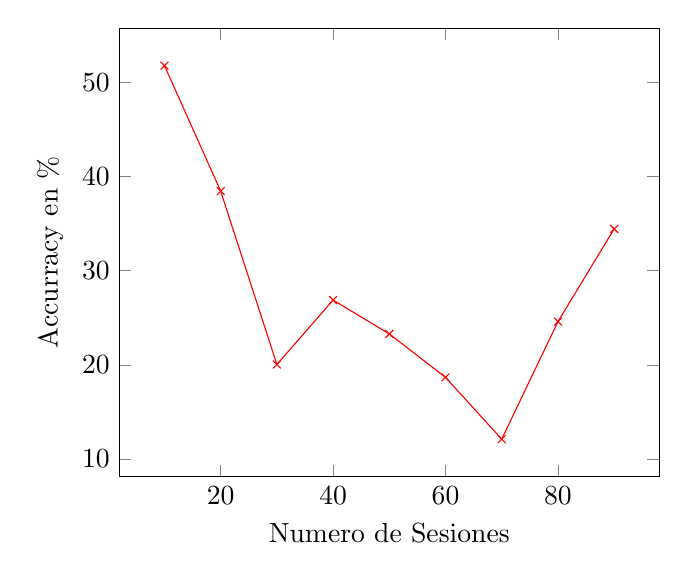
\begin{tikzpicture}
	\begin{axis}[
	xlabel= Numero de Sesiones,
	ylabel=Accurracy en \% ]
	\addplot[color=red,mark=x] coordinates {
		(10, 51.77777778)
		(20, 38.44444444)
		(30, 20.03448276)
		(40, 26.87179487)
		(50, 23.28)
		(60, 18.66666667)
		(70, 12.1)
		(80, 24.5875)
		(90, 34.43333333)
	};
	\end{axis}
	\end{tikzpicture}
	
	
	
	
	
	
	
	
	\item Sesiones con mas de 10 webaccess para generar el Trie


	
\end{enumerate}











Lo que se busca es ver como se comporta el algoritmo con datos discretos de cinco símbolos o más, es decir sesiones de usuarios que por lo menos han visitado cinco secciones de una web. Aquí se mide también lo estocástico de cada evento. 





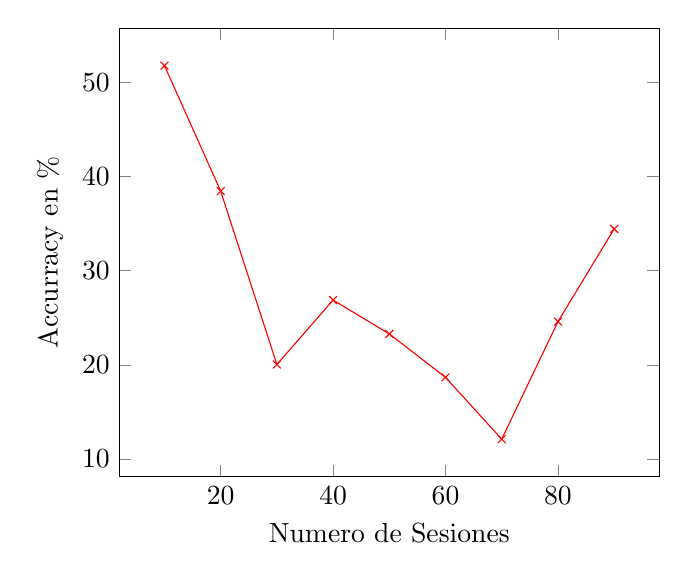
\begin{tikzpicture}
	\begin{axis}[
	xlabel= Numero de Sesiones,
	ylabel=Accurracy en \% ]
		\addplot[color=red,mark=x] coordinates {
			(10, 51.77777778)
			(20, 38.44444444)
			(30, 20.03448276)
			(40, 26.87179487)
			(50, 23.28)
			(60, 18.66666667)
			(70, 12.1)
			(80, 24.5875)
			(90, 34.43333333)
		};
	\end{axis}
\end{tikzpicture}







	% \begin{forest} 
	% 	[VP
	% 	[DP]
	% 	[V’
	% 	[V]
	% 	[DP]
	% 	]
	% 	]
	% \end{forest}



	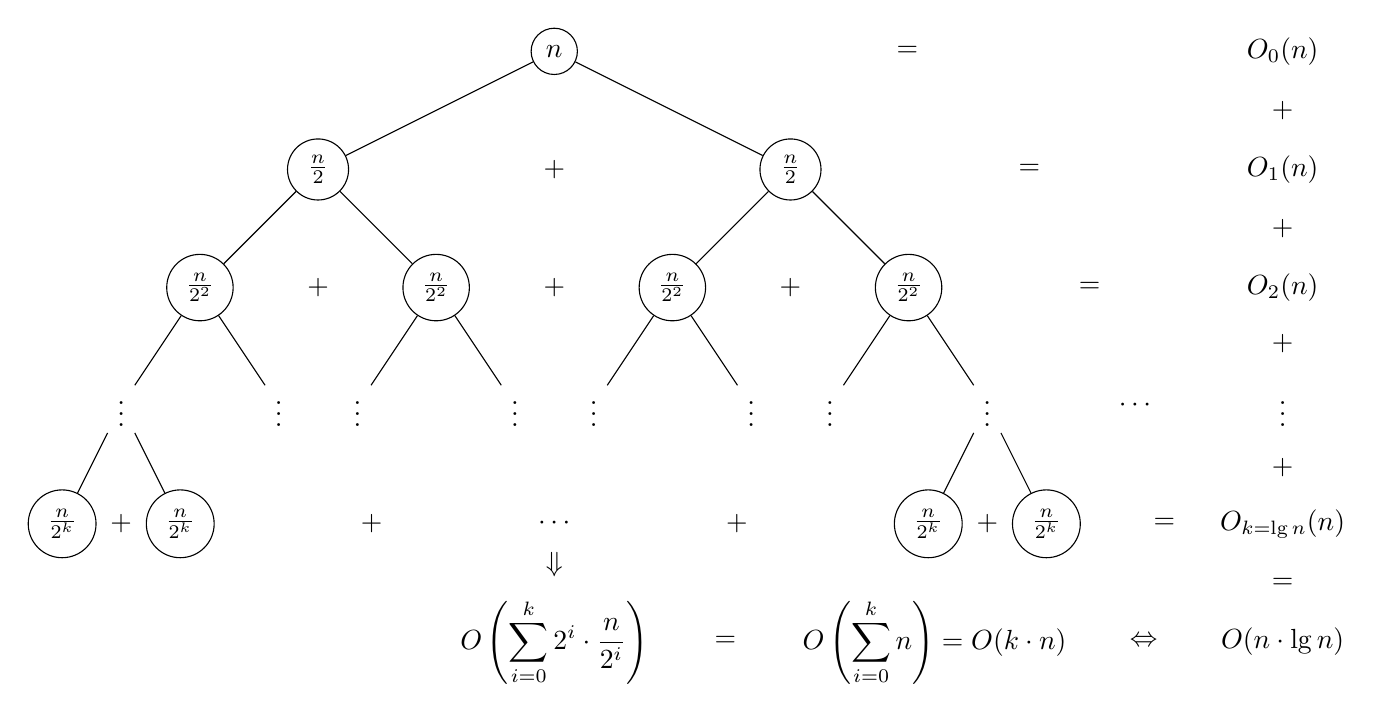
\begin{tikzpicture}[level/.style={sibling distance=60mm/#1}]
	\node [circle,draw] (z){$n$}
	child {node [circle,draw] (a) {$\frac{n}{2}$}
		child {node [circle,draw] (b) {$\frac{n}{2^2}$}
			child {node {$\vdots$}
				child {node [circle,draw] (d) {$\frac{n}{2^k}$}}
				child {node [circle,draw] (e) {$\frac{n}{2^k}$}}
			} 
			child {node {$\vdots$}}
		}
		child {node [circle,draw] (g) {$\frac{n}{2^2}$}
			child {node {$\vdots$}}
			child {node {$\vdots$}}
		}
	}
	child {node [circle,draw] (j) {$\frac{n}{2}$}
		child {node [circle,draw] (k) {$\frac{n}{2^2}$}
			child {node {$\vdots$}}
			child {node {$\vdots$}}
		}
		child {node [circle,draw] (l) {$\frac{n}{2^2}$}
			child {node {$\vdots$}}
			child {node (c){$\vdots$}
				child {node [circle,draw] (o) {$\frac{n}{2^k}$}}
				child {node [circle,draw] (p) {$\frac{n}{2^k}$}
					child [grow=right] {node (q) {$=$} edge from parent[draw=none]
						child [grow=right] {node (q) {$O_{k = \lg n}(n)$} edge from parent[draw=none]
							child [grow=up] {node (r) {$\vdots$} edge from parent[draw=none]
								child [grow=up] {node (s) {$O_2(n)$} edge from parent[draw=none]
									child [grow=up] {node (t) {$O_1(n)$} edge from parent[draw=none]
										child [grow=up] {node (u) {$O_0(n)$} edge from parent[draw=none]}
									}
								}
							}
							child [grow=down] {node (v) {$O(n \cdot \lg n)$}edge from parent[draw=none]}
						}
					}
				}
			}
		}
	};
	\path (a) -- (j) node [midway] {+};
	\path (b) -- (g) node [midway] {+};
	\path (k) -- (l) node [midway] {+};
	\path (k) -- (g) node [midway] {+};
	\path (d) -- (e) node [midway] {+};
	\path (o) -- (p) node [midway] {+};
	\path (o) -- (e) node (x) [midway] {$\cdots$}
	child [grow=down] {
		node (y) {$O\left(\displaystyle\sum_{i = 0}^k 2^i \cdot \frac{n}{2^i}\right)$}
		edge from parent[draw=none]
	};
	\path (q) -- (r) node [midway] {+};
	\path (s) -- (r) node [midway] {+};
	\path (s) -- (t) node [midway] {+};
	\path (s) -- (l) node [midway] {=};
	\path (t) -- (u) node [midway] {+};
	\path (z) -- (u) node [midway] {=};
	\path (j) -- (t) node [midway] {=};
	\path (y) -- (x) node [midway] {$\Downarrow$};
	\path (v) -- (y)
	node (w) [midway] {$O\left(\displaystyle\sum_{i = 0}^k n\right) = O(k \cdot n)$};
	\path (q) -- (v) node [midway] {=};
	\path (e) -- (x) node [midway] {+};
	\path (o) -- (x) node [midway] {+};
	\path (y) -- (w) node [midway] {$=$};
	\path (v) -- (w) node [midway] {$\Leftrightarrow$};
	\path (r) -- (c) node [midway] {$\cdots$};
	\end{tikzpicture}



%Las conclusiones son deducidas logicamen- te de los resultados obtenidos y de la interpretacionpresen- tada, ademas estan conectadas al marco teorico.
%Las conclusiones muestran el logro de los ob jetivos.
%Se presentan proyec- ciones validas y valio- sas a partir del traba- jo realizado.
%Se detallan claramen- te las limitaciones del traba jo realizado.














\subsection{Experimento con Largo de Ventana}

	Cual podria ser el optimo de la ventana
	Que ventana o cual corre mejor



\subsection{Experimento con el Tamaño del Set de datos de Entrenamiento}


\subsection{Experimento con Predicciones con Ruido}




\subsection{Cross Validation}


\subsection{Accurracy}



\subsection{Precisión}


	% Es una métrica que captura una porición correcta de toda la data a probar. 
	% Una manera de modelar esto es para cada consulta que hacemos al predictor, damos un score de 1 y 0, luego podemos tomar el promedio de este score.
	
	
	
	% PredictionIO has a [[AverageMetric]] helper class which provides this feature. This class takes 4 type parameters, [[EvalInfo]], [[Query]], [[PredictedResult]], and [[ActualResult]], these types can be found from the engine's signature. Line 5 below is the custom calculation.
	
	 %Precision is a metric for binary classifier capturing the portion of correction prediction among all positive predictions. We don't care about the cases where the QPA-tuple gives a negative prediction. (Recall that a binary classifier only provide two output values: positive and negative.) The following table illustrates all four cases:
	 
	 %Calculating the precision metric is a slightly more involved procedure than calculating the accuracy metric as we have to specially handle the don't care negative cases.
	 
	 %x PredictionIO provides a helper class OptionAverageMetric allows user to specify don't care values as None. It only aggregates the non-None values. Lines 3 to 4 is the method signature of calcuate method. The key difference is that the return value is a Option[Double], in contrast to Double for AverageMetric. This class only computes the average of Some(.) results. Lines 5 to 13 are the actual logic. The first if factors out the positively predicted case, and the computation is simliar to the accuracy metric. The negatively predicted case are the don't cares, which we return None.
	 
	 % \subsection{Experimento comparativo con Frequent Sequency Pattern}
	 
	 
	 %\subsection{Decission Tree}
	 %\subsection{Asociation Rulz}
	








\section{Conclusiones y Resultados}



%In this paper we studied the empirical performance of a number of prominent prediction algorithms. We focused on prediction settings that are more closely related to those required

%%%%%%%%% On Prediction Using Variable Order Markov Models

%$%%%%%%%%
%%n this paper we studied the empirical performance of a number of prominent prediction algorithms. We focused on prediction settings that are more closely related to those required
%On Prediction Using Variable Order Markov Models
%by machine learning practitioners dealing with discrete sequences.
%However, somewhat surprisingly, the best predictor under the log-loss is not the best classifier. On the contrary, the consistently best protein classifier is based on the mediocre lz-ms predictor! This algo- rithm is a simple modification of the well-known Lempel-Ziv-78 (lz78) prediction algorithm, which can capture VMMs with large contexts. The surprisingly good classification accuracy achieved by this algorithm may be of independent interest to protein analysis research and clearly deserves further investigatio 
% Genero toda las referencias para demostrar el uso de la bibliografía
% No es necesario que utilice este comando en su document
%
%Conclusion of this paper Gopalratnam Cook
%alz effectively models sequential processes, and is extremely useful for prediction of processes where events are dependent on the previous event history. This is because of the ability of the algorithm to build an accurate model of the source of the events being generated, a feature inherited from its information theoretic background and the LZ78 text compression algorithm. 
%The effectiveness of the method for learning a measure of time can also be attributed to fact that ALZ is a strong sequential predictor. The sound theoretical principles on which ALZ is founded also mean that ALZ is an optimal Universal Predictor, and can be used in a variety of prediction scenarios.
%conclusion lcoa
%Dado que la myora de los predictores funcionan de 
%manera offline, uno de los aporte de tener estar estructura de algoritmos como servicios es poder tener un motor de prediccion en linea.
